\documentclass[a4paper]{article}
\usepackage[utf8]{inputenc}
\usepackage[english,russian]{babel}
\usepackage{hyperxmp}
\usepackage{titling}
\usepackage[colorlinks,linkcolor=blue]{hyperref}
\usepackage{graphicx}
\usepackage{fancyhdr}
\usepackage{a4wide}
\usepackage{xspace}
\usepackage{lastpage}
\usepackage{ccicons}
\usepackage{wrapfig}
\usepackage{multicol}

\newcommand{\myhref}[2]{{\href{#1}{\textcolor{blue}{#2}}}}

\fancyhead[L]{\thetitle}
\fancyhead[R]{\it\thepage\ of \pageref{LastPage}}
%\fancyfoot[C]{\centerline{\small \ccbysa\ \theauthor, 2013. This work is licensed under a \myhref{http://creativecommons.org/licenses/by-sa/3.0/}{Creative Commons Attribution-ShareAlike 3.0 Unported License.}}}
\pagestyle{fancy}

%% PDF meta-data
\hypersetup{%
pdftitle={Assigment 2 for the course on city design. Three Special Places.}
pdfauthor={Vitaly Repin},
pdfcopyright={This work is licensed under a Creative Commons Attribution-ShareAlike 3.0 Unported License},
pdfsubject={Designing City},
pdfkeywords={design,city,map,places},
pdflicenseurl={http://creativecommons.org/licenses/by-sa/3.0/},
pdfcaptionwriter={Vitaly Repin},
pdfcontactcity={Espoo},
pdfcontactcountry={Finland},
pdfcontactemail={vitaly.repin@gmail.com},
pdflang={en}
}

%% City name
\newcommand{\mycity}{St. Petersburg, Russia\xspace}
%% Author
\author{Vitaly Repin}
%% Title
\title{Three Special Places: \emph{\mycity}}

\date{November, 2013}

\begin{document}
{\section{Street: Улица Зодчего Росси (\myhref{http://goo.gl/maps/C3ZED}{Rossi Street})}
\begin{wrapfigure}{l}{.5\textwidth}
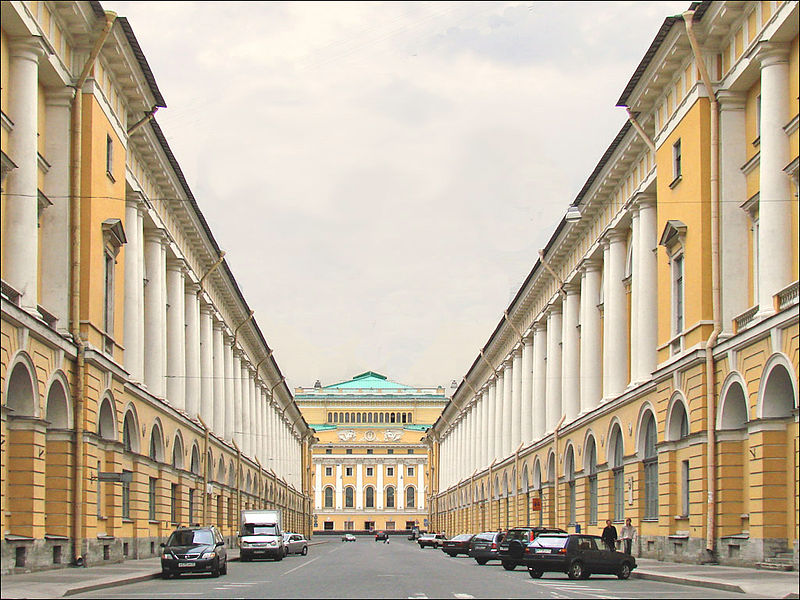
\includegraphics[keepaspectratio,width=.5\textwidth]{Rossi1}
\textit{Rossi Street. XXI century.}
\end{wrapfigure}

Rossi street is one of the most beautiful streets in the city of St. Petersburg. It's pretty short and
consists of five buildings. But these buildings are designed with
the similar facades and that's why these buildings are seen as one building, one facade.

This view is very impressive and attracts a lot of people - tourists from all over the world as well as locals.
The street follows the antique canons: its width equals to the height of the buildings located on the street (22 meters) and its length is 10 times longer (220 meters).

Rossi Street connects two small squares - Lomonosova square and Orstrovskogo square.
This street was built in 1824--1834. The author of the project was a famous architect of the time ---
\myhref{http://en.wikipedia.org/wiki/Carlo_Rossi_(architect)}{Carlo Rossi.}

\begin{wrapfigure}{r}{.5\textwidth}
\vspace*{-.5cm}
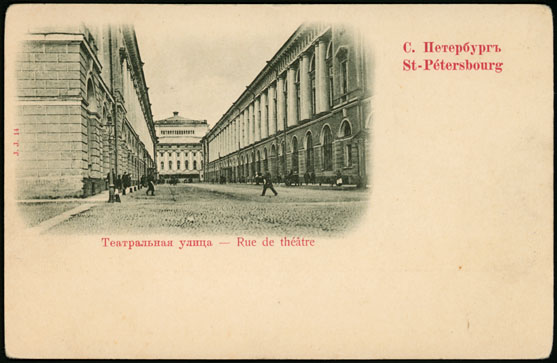
\includegraphics[keepaspectratio,width=.5\textwidth]{Rossi2}
\textit{Rossi Street. Beginning of the XX century.}
\end{wrapfigure}
The street was so perfectly designed that
there was no need to change it and currently we see almost the same view as in the time of its completion.

Rossi street is mostly used by artists. \myhref{http://en.wikipedia.org/wiki/Vaganova_Academy_of_Russian_Ballet}{Vaganova Academy of Russian Ballet},
\myhref{http://www.theatremuseum.ru/en/mtm_abt.html}{St. Petersburg State Museum of Theatre and Music},
\myhref{http://sptl.spb.ru/?lang=en}{St. Petersburg State Theater Library} are located there (as well as several govermental offices).

\begin{tabular}{lp{.7\textwidth}}
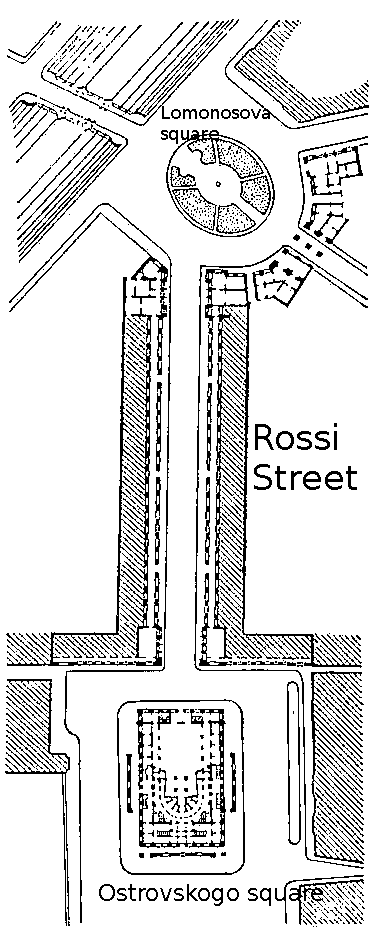
\includegraphics[keepaspectratio,width=.2\textwidth]{rossiplan}&\raisebox{3.8cm}{\begin{minipage}{.7\textwidth}\myhref{http://en.wikipedia.org/wiki/Alexandrinsky_Theatre}{Alexandrinsky Theater} is located at Ostrovskogo square and its famous building (which  is part of
the UNESCO World Heritage Site) is clearly seen if you are walking by Rossi street. I think it's fair to say that Rossi Street represents a perfect match 
between form and function. The form is very aesthetic and it is in a perfect harmony with the function of this street --- be home for artists.\\ The street is located in historical center of St. Petersburg, ex-capital of Russia, and in a walking distance from the main promenade place in the city --- Nevsky prospect. It also contributes to the success of the street.\end{minipage}}
\end{tabular}}
\newpage

\section*{Public space: Площадь Искусств (\myhref{http://goo.gl/maps/mRfWG}{Arts Square})}

\begin{tabular}{ll}
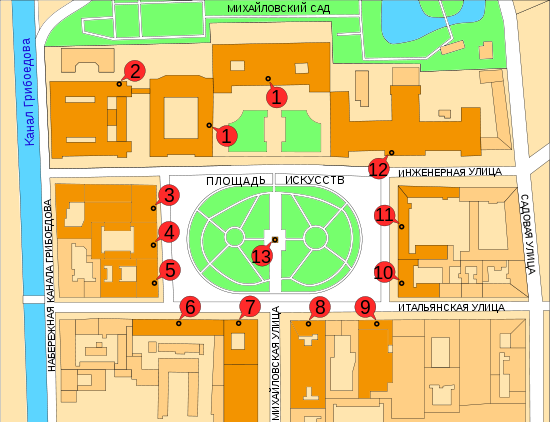
\includegraphics[keepaspectratio,width=.48\textwidth]{artsqplan}&
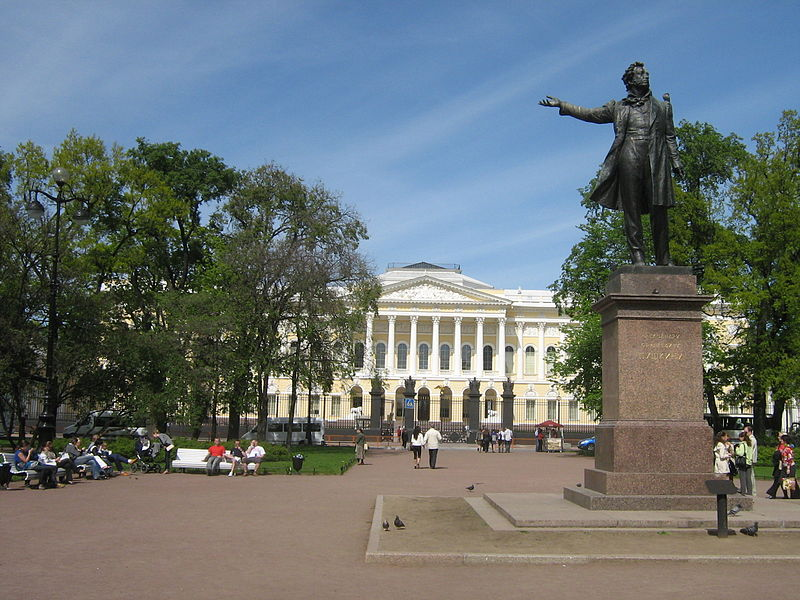
\includegraphics[keepaspectratio,width=.48\textwidth]{pushkin}
\end{tabular}

Arts square is located in the historical city center of St. Petersburg. It is surrounded by nice
\begin{wrapfigure}{l}{.4\textwidth}
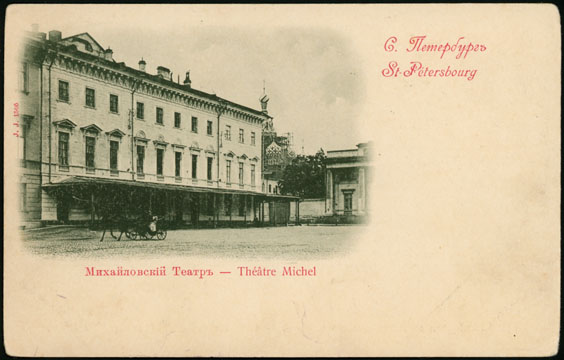
\includegraphics[keepaspectratio,width=.4\textwidth]{opera}
\textit{Mikhaylovsky Theater, beginning of the XX century}
\vspace*{-.3cm}
\end{wrapfigure}
buildings. Most of them are used for the artistic purposes (museums
and theaters). There is a small garden in the center of the square. Monument to the famous Russian poet Alexander Pushkin was installed in the heart of this garden in 1957.

Nice views, artistic atmosphere and the beautiful garden in the center of the square make this place a center of attraction for a lot of locals and tourists. Especially in the summer time.
But the square is full of people all year around because of the buildings which are forming it. It lives the life of Art events all the year.

The square was designed by \myhref{http://en.wikipedia.org/wiki/Carlo_Rossi_(architect)}{Carlo Rossi} in 1825. Different architects were participating in the
development of the square. E.g, Mikhailovsky Theatre (item 3 in the plan, built in 1833) was designed by \href{http://en.wikipedia.org/wiki/Alexander_Brullov}{Brullov}
and \myhref{http://en.wikipedia.org/wiki/Carlo_Rossi_(architect)}{Rossi}; the garden in the center of the square was designed by Rossi and Bush (according to the
tradition of English landscape parks). A lot of other architects developed the square further. But the main ideas proposed by Rossi were respected through all
the square history. Architects tried to keep "Rossi's style".

\medskip
\centerline{\large\bf Buildings located in the square}

\begin{multicols}{2}
\begin{enumerate}
\item Mikhailovsky Palace (\myhref{http://en.wikipedia.org/wiki/Russian_Museum}{Russian Museum} is located there)
\item Mikhailovsky Palace, Benois Wing (\myhref{http://en.wikipedia.org/wiki/Russian_Museum}{Russian Museum} is located there)
\item \myhref{http://en.wikipedia.org/wiki/Mikhaylovsky_Theatre}{Mikhaylovsky Theatre}
\item \myhref{http://www.encspb.ru/object/2804024725?lc=en}{Golenischev-Kutuzov's house}
\item Zhako's house
\item House belonging to the \myhref{http://en.wikipedia.org/wiki/Catholic_Church_of_St._Catherine}{Catholic Church of St. Catherine}
\item \myhref{http://en.wikipedia.org/wiki/Grand_Hotel_Europe}{Hotel "Europe"}
\item \myhref{http://en.wikipedia.org/wiki/Saint_Petersburg_Philharmonia}{St. Petersburg Philharmonia, Grand Hall}
\item \myhref{http://spbmuzcomedy.com/en/}{St. Petersburg Theatre of Musical Comedy}
\item Vielgorsky's house (Part of the building is occupied by the Russian Museum now)
\item School (belongs to the Russian Museum)
\item \myhref{http://en.wikipedia.org/wiki/Russian_Museum_of_Ethnography}{Russian Museum of Ethnography}
\item \myhref{http://www.saint-petersburg.com/monuments/alexander-pushkin/}{Monument to Alexander Pushkin}
\end{enumerate}
\end{multicols}
\newpage

\section{District: Заячий остров (\myhref{http://goo.gl/maps/KJ6t2}{Hare Island})}

\includegraphics[keepaspectratio,width=.48\textwidth]{paul}\hspace{.2cm}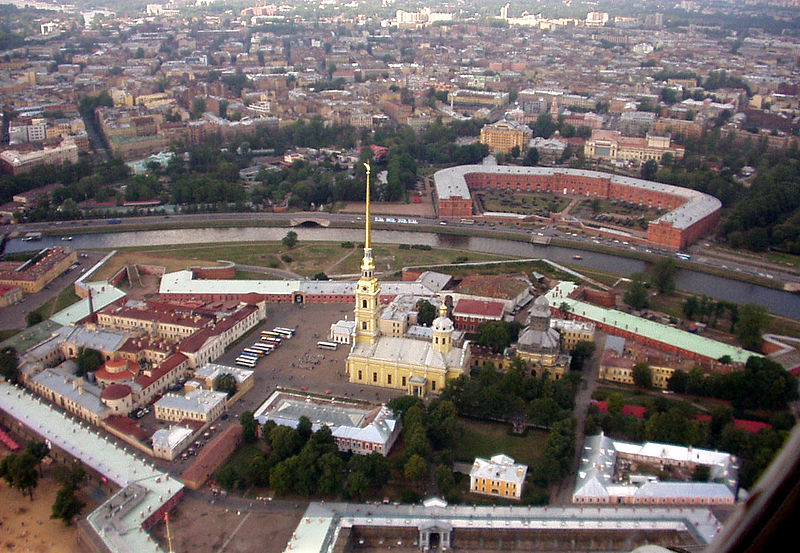
\includegraphics[keepaspectratio,width=.48\textwidth]{paul2}

\myhref{http://en.wikipedia.org/wiki/Zayachy_Island}{Hare Island} is one of the most famous districts of St. Petersburg. This is the place where the city was founded
in 1703. \myhref{http://en.wikipedia.org/wiki/Peter_and_Paul_fortress}{Peter and Paul Fortress} was the first building there.\\
\begin{wrapfigure}{l}{.49\textwidth}
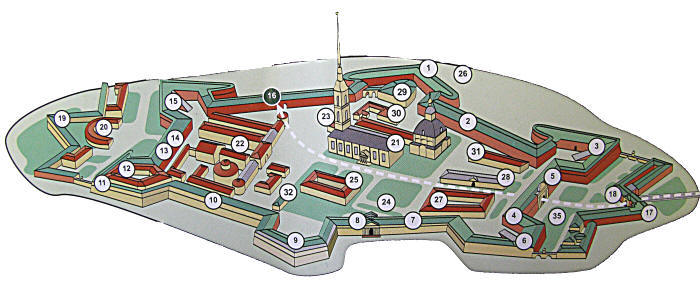
\includegraphics[keepaspectratio,width=.48\textwidth]{planpetr}
\end{wrapfigure}
It still occupies most of the space on the island. The role of the island was different in the different historical periods.

Originally it served military purpose (defence of the new Russian capital from Sweden) but with time it lost this meaning. It was a prison for the state
political prisoners most of the time. 

Dominant of the island is the \myhref{http://en.wikipedia.org/wiki/Peter_and_Paul_Cathedral}{Peter and Paul cathedral.} It played an important role in the
capital as it houses the remains of almost all the Russian Emperors and Empresses from Peter the Great to Nicholas II and his family.

\myhref{http://en.wikipedia.org/wiki/Domenico_Trezzini}{Domenico Trezzini} designed the fortress and the Cathedral.

Nowadays the place is mostly a museum (however, there is one apartment house in the island). Cultural heritage attracts the tourists from all over the world.
Locals and tourists are also enjoying the beach located in the island which is probably the most famous beach of St. Petersburg. It's very popular regardless
of the fact that the water in Neva river is polluted and not suitable for swimming. Most of the people just enjoy sunlight on the beach in the heart of the city.

Hare island is pretty busy with a lot of exhibitions and art events. Especially during summer time. They also attract people to this place. It provides a rest from the
busy city life just in the very heart of the city!
\end{document}
